\documentclass{article}
\usepackage[utf8]{inputenc} % para que nos acepte la codificación UTF-8
\usepackage[spanish]{babel} % establecemos el idioma del documento al español
\usepackage{graphicx,float}
\begin{document}

\title{Relacion de ejercicios MC. Practica 2}
\author{Pablo Navarro}
\maketitle
\begin{enumerate}
  \item  Dibuja los AFDs que aceptan los siguientes lenguajes con alfabeto {0,1}:
  \begin{itemize}
    \item [a)] El lenguaje \{11,00\}
          \begin{figure}[H]
            \centering
            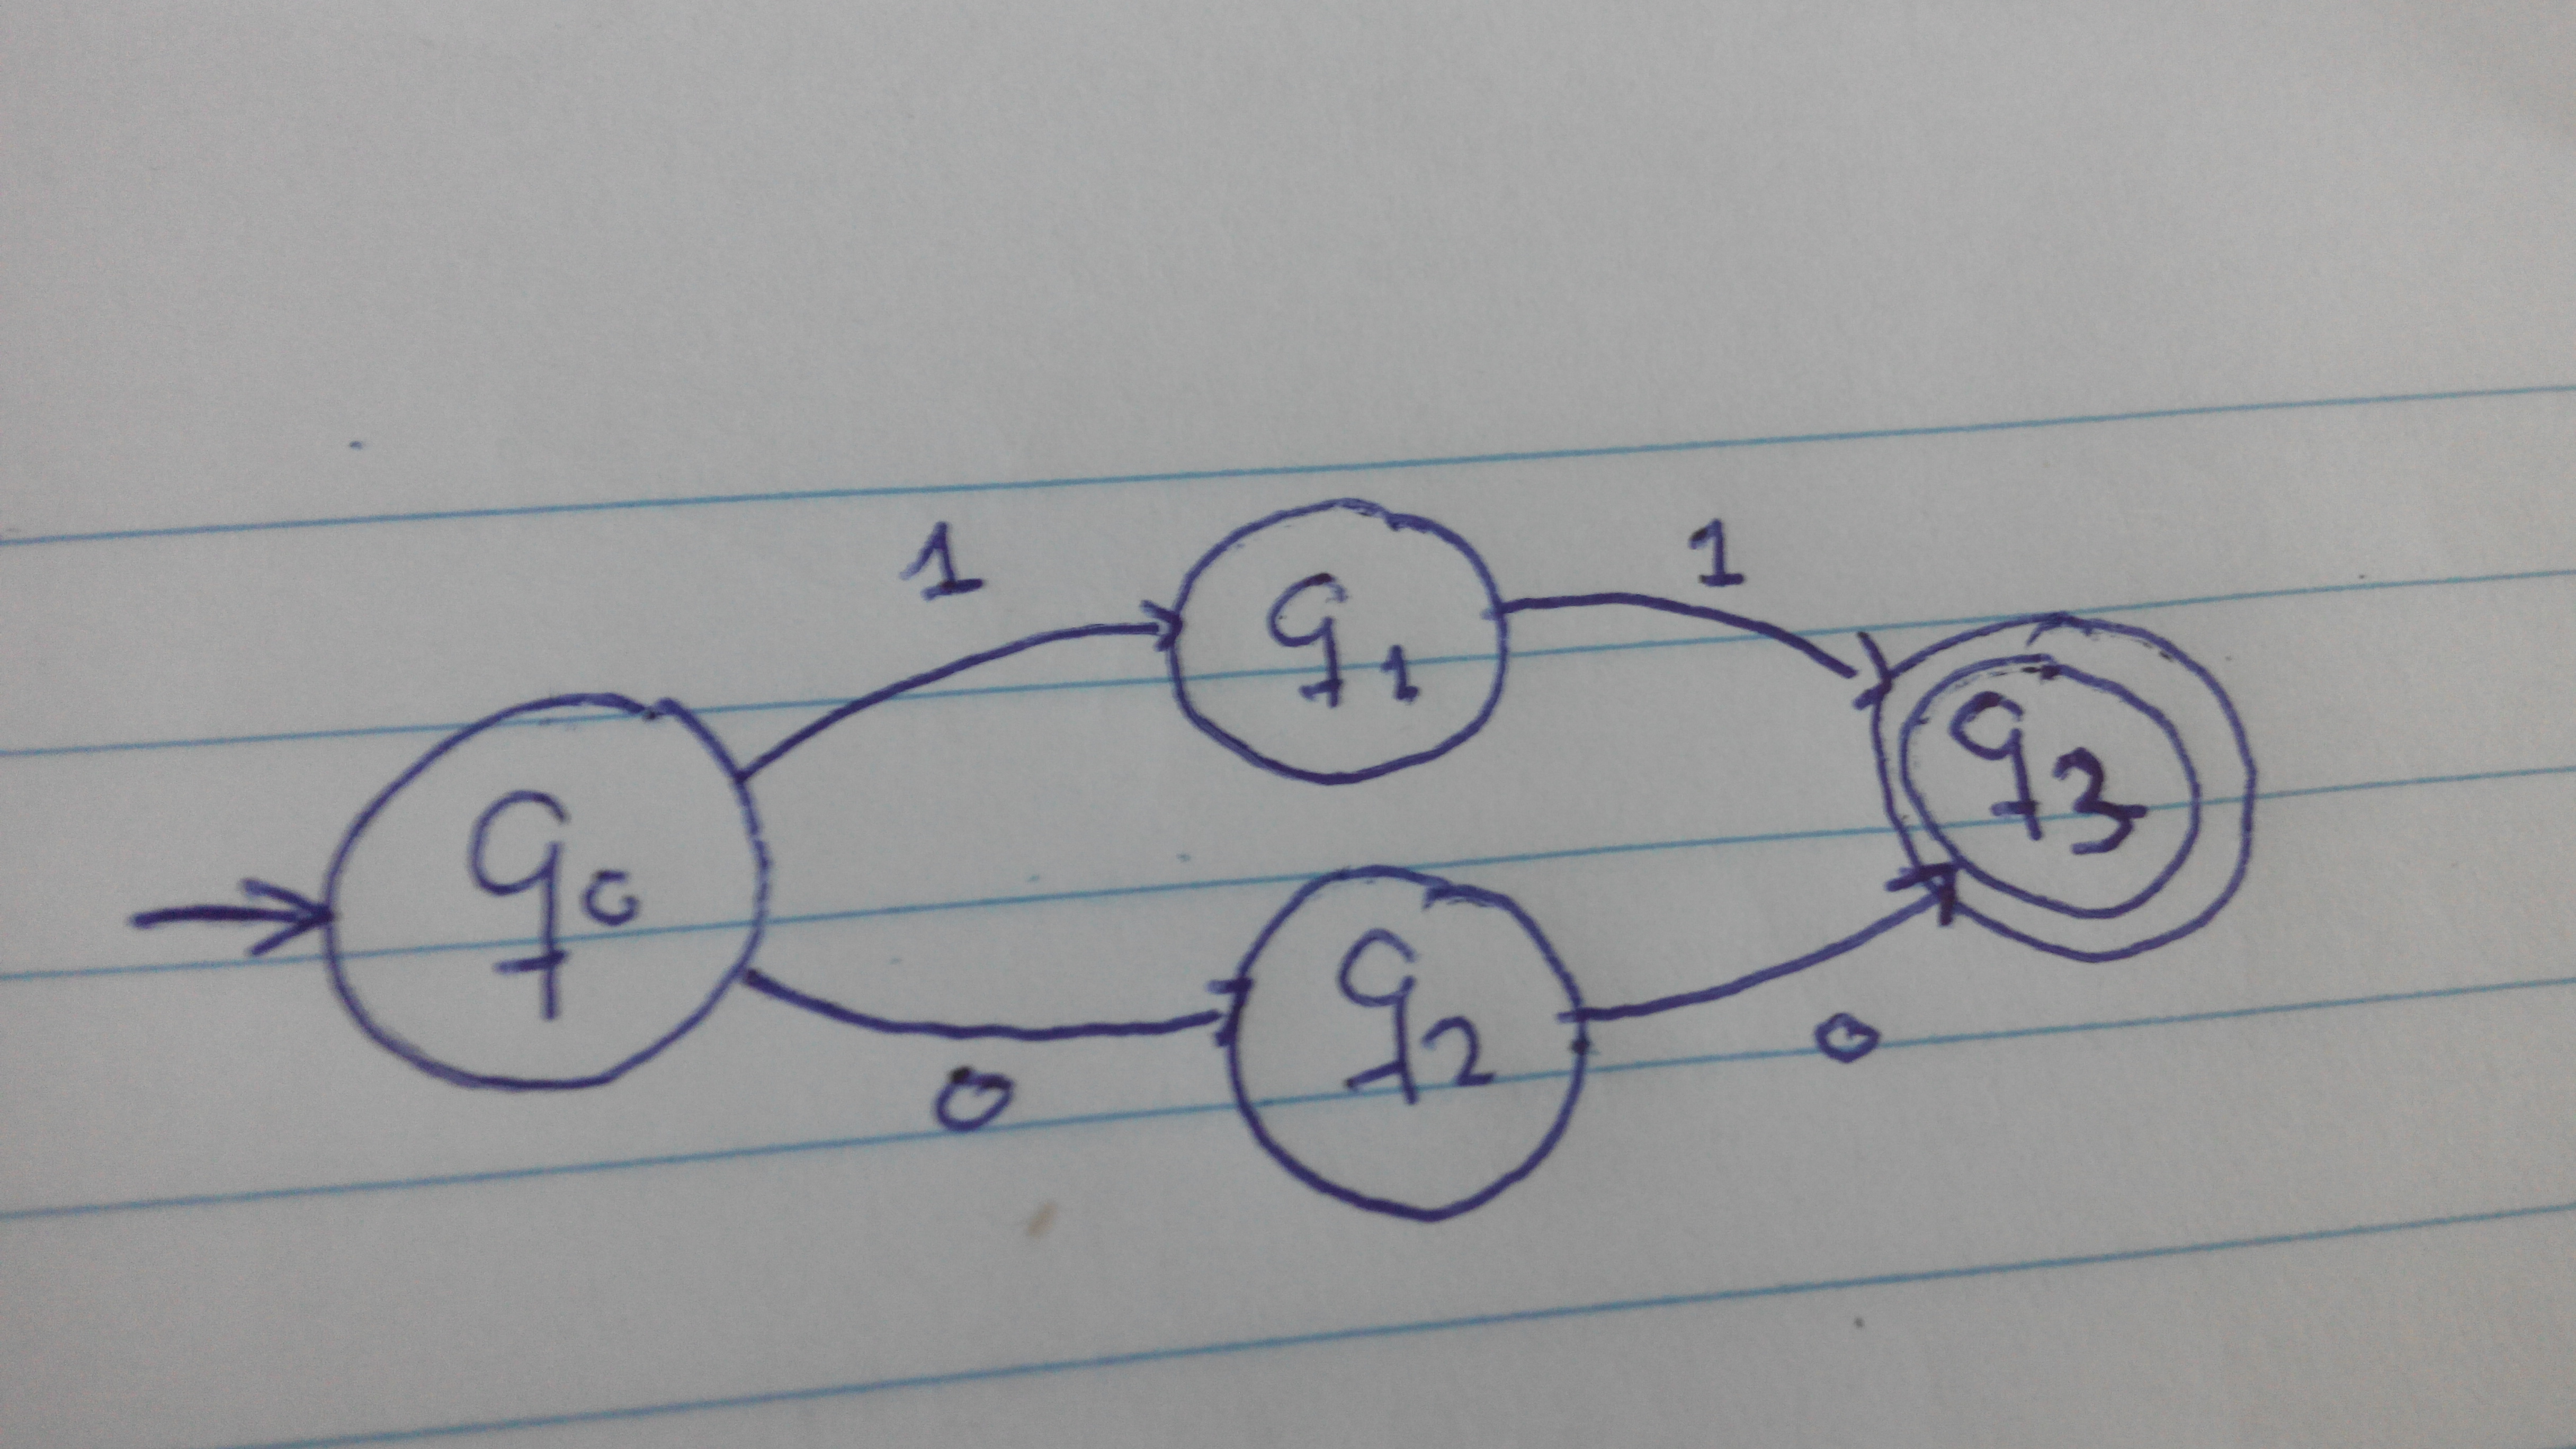
\includegraphics[width=7cm, height=5cm]{1a}
          \end{figure}
    \item [b)] El lenguaje formado por las cadenas donde el número de ceros es
divisible por 3.
          \begin{figure}[H]
            \centering
            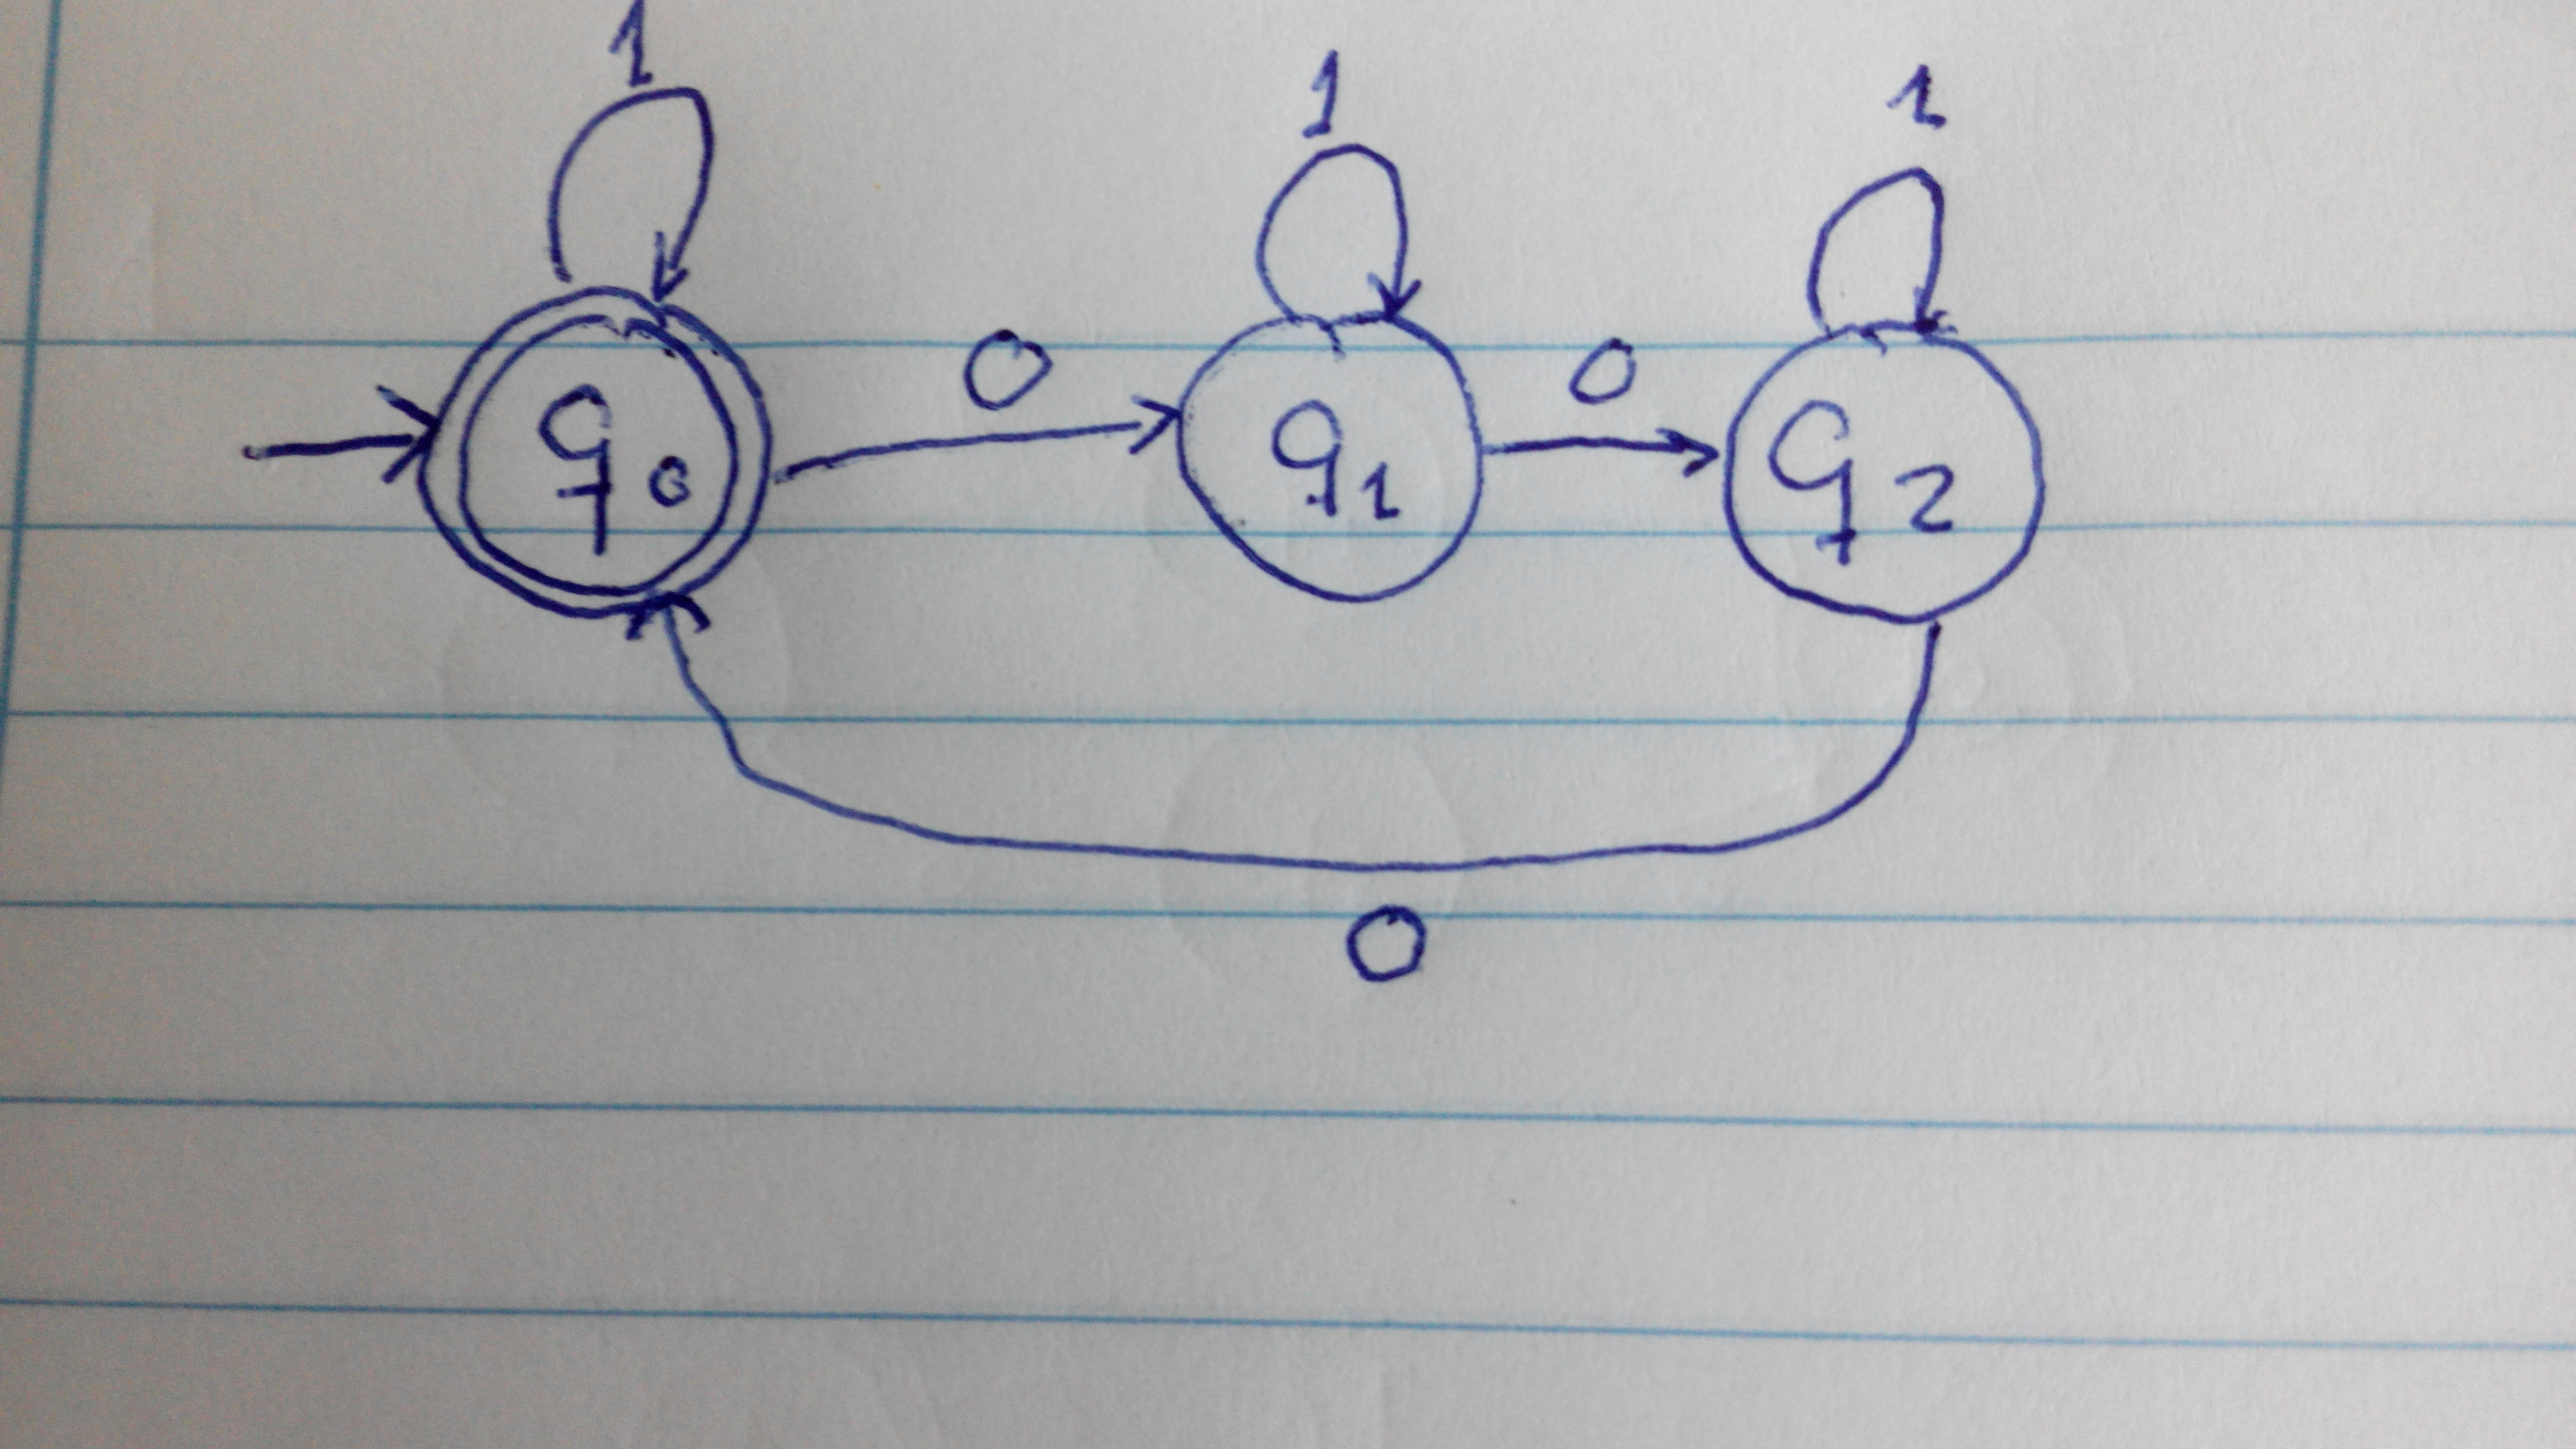
\includegraphics[width=7cm, height=5cm]{1b}
          \end{figure}
    \item [c)] El lenguaje de las palabras que contienen la subcadena 11.
          \begin{figure}[H]
            \centering
            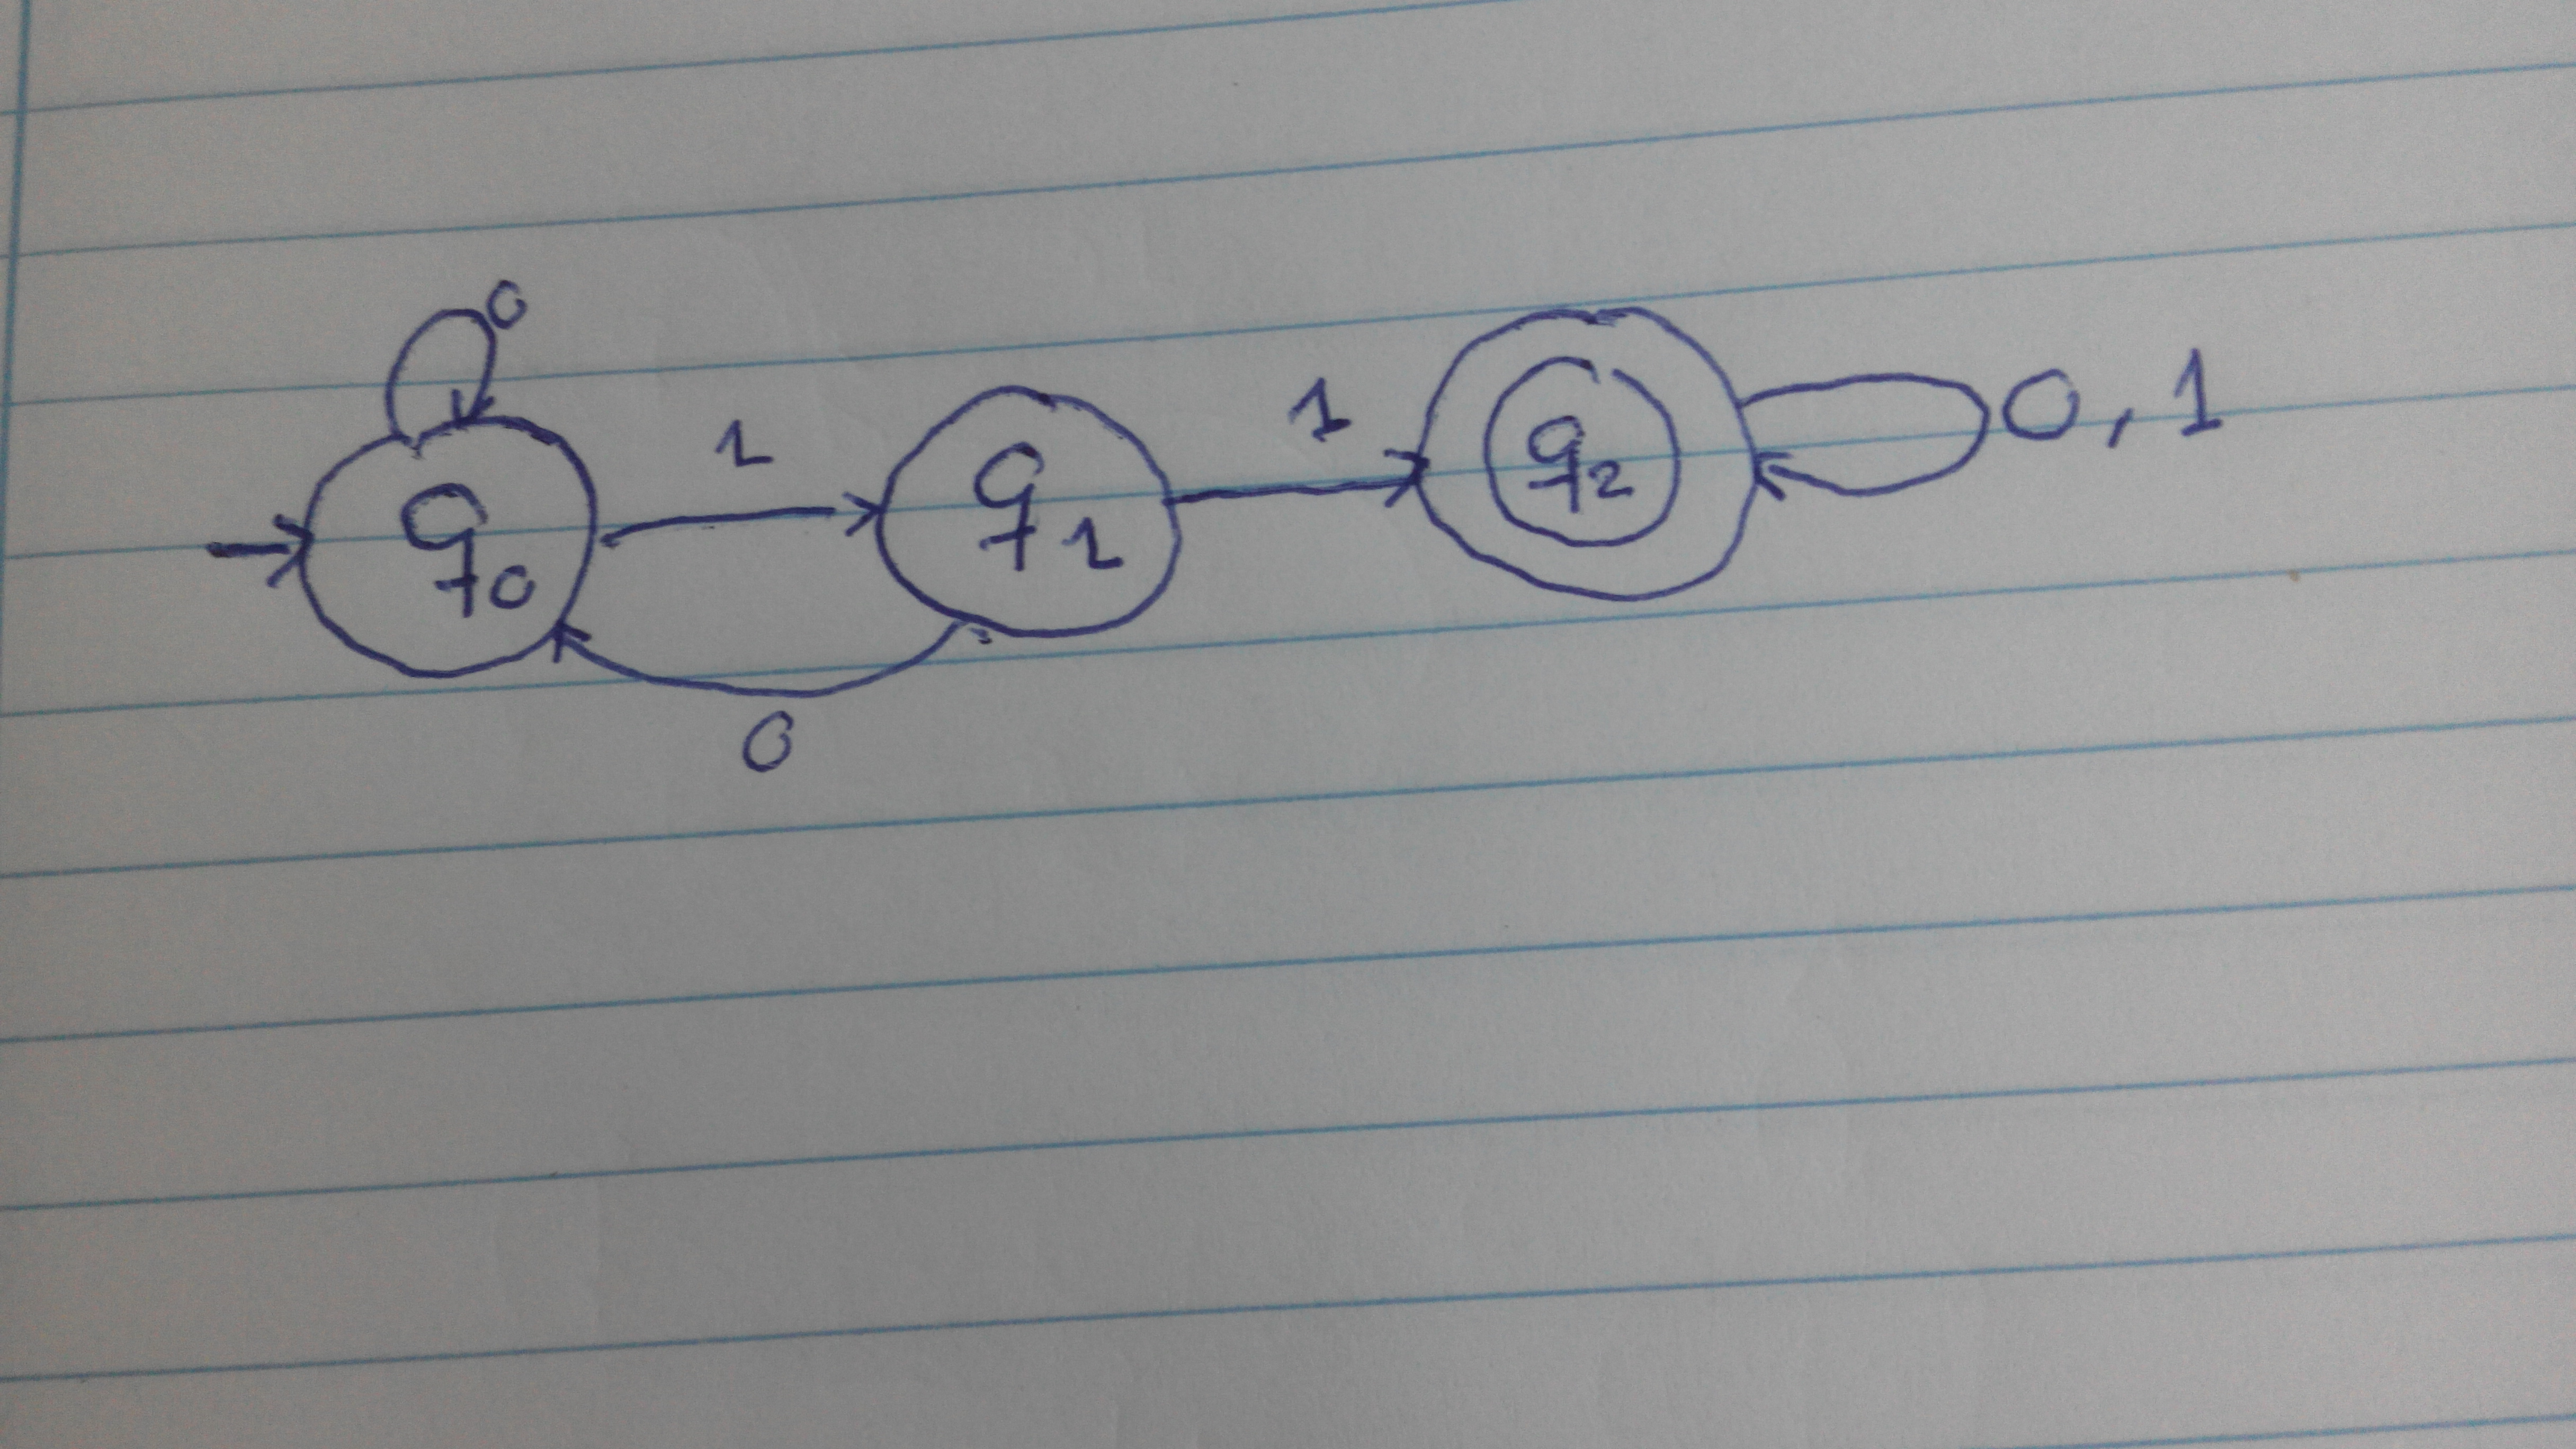
\includegraphics[width=7cm, height=5cm]{1c}
          \end{figure}
    \item [d)] El lenguaje de las palabras que empiezan o terminan (o ambas cosas) en
11.
          \begin{figure}[H]
            \centering
            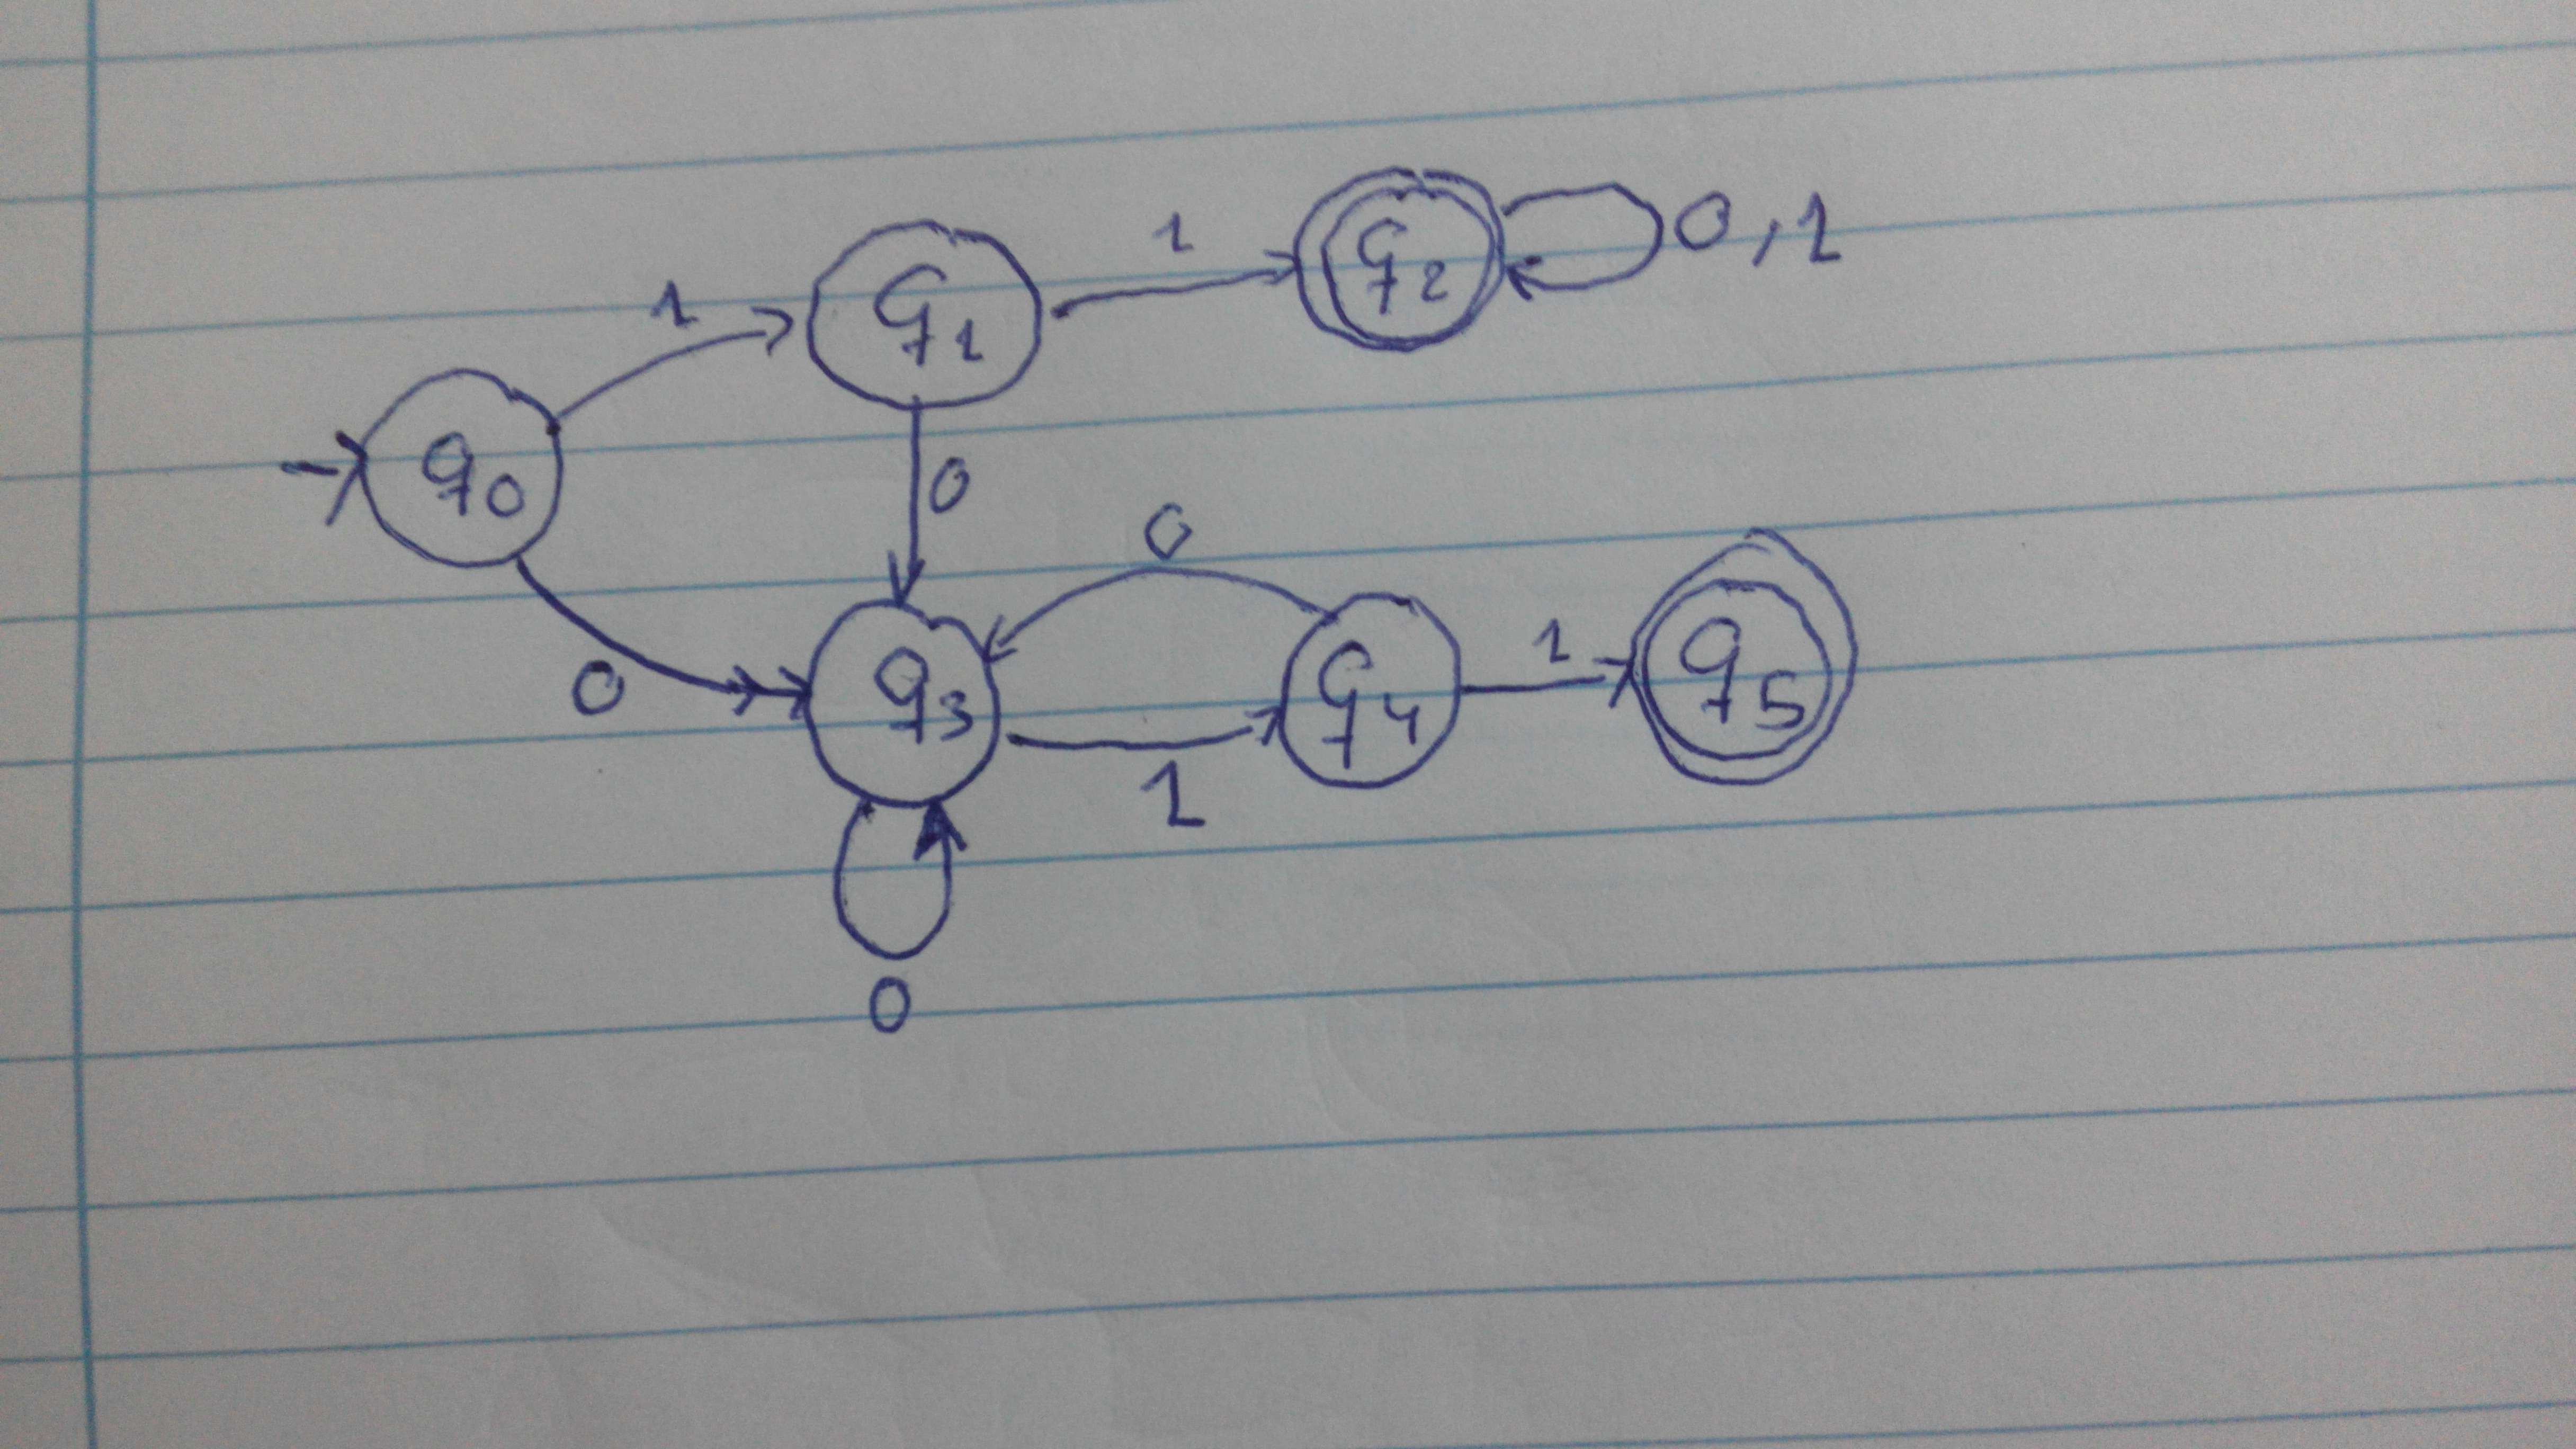
\includegraphics[width=7cm, height=5cm]{1d}
          \end{figure}
  \end{itemize}
  \item [2]·
        \begin{figure}[H]
          \centering
          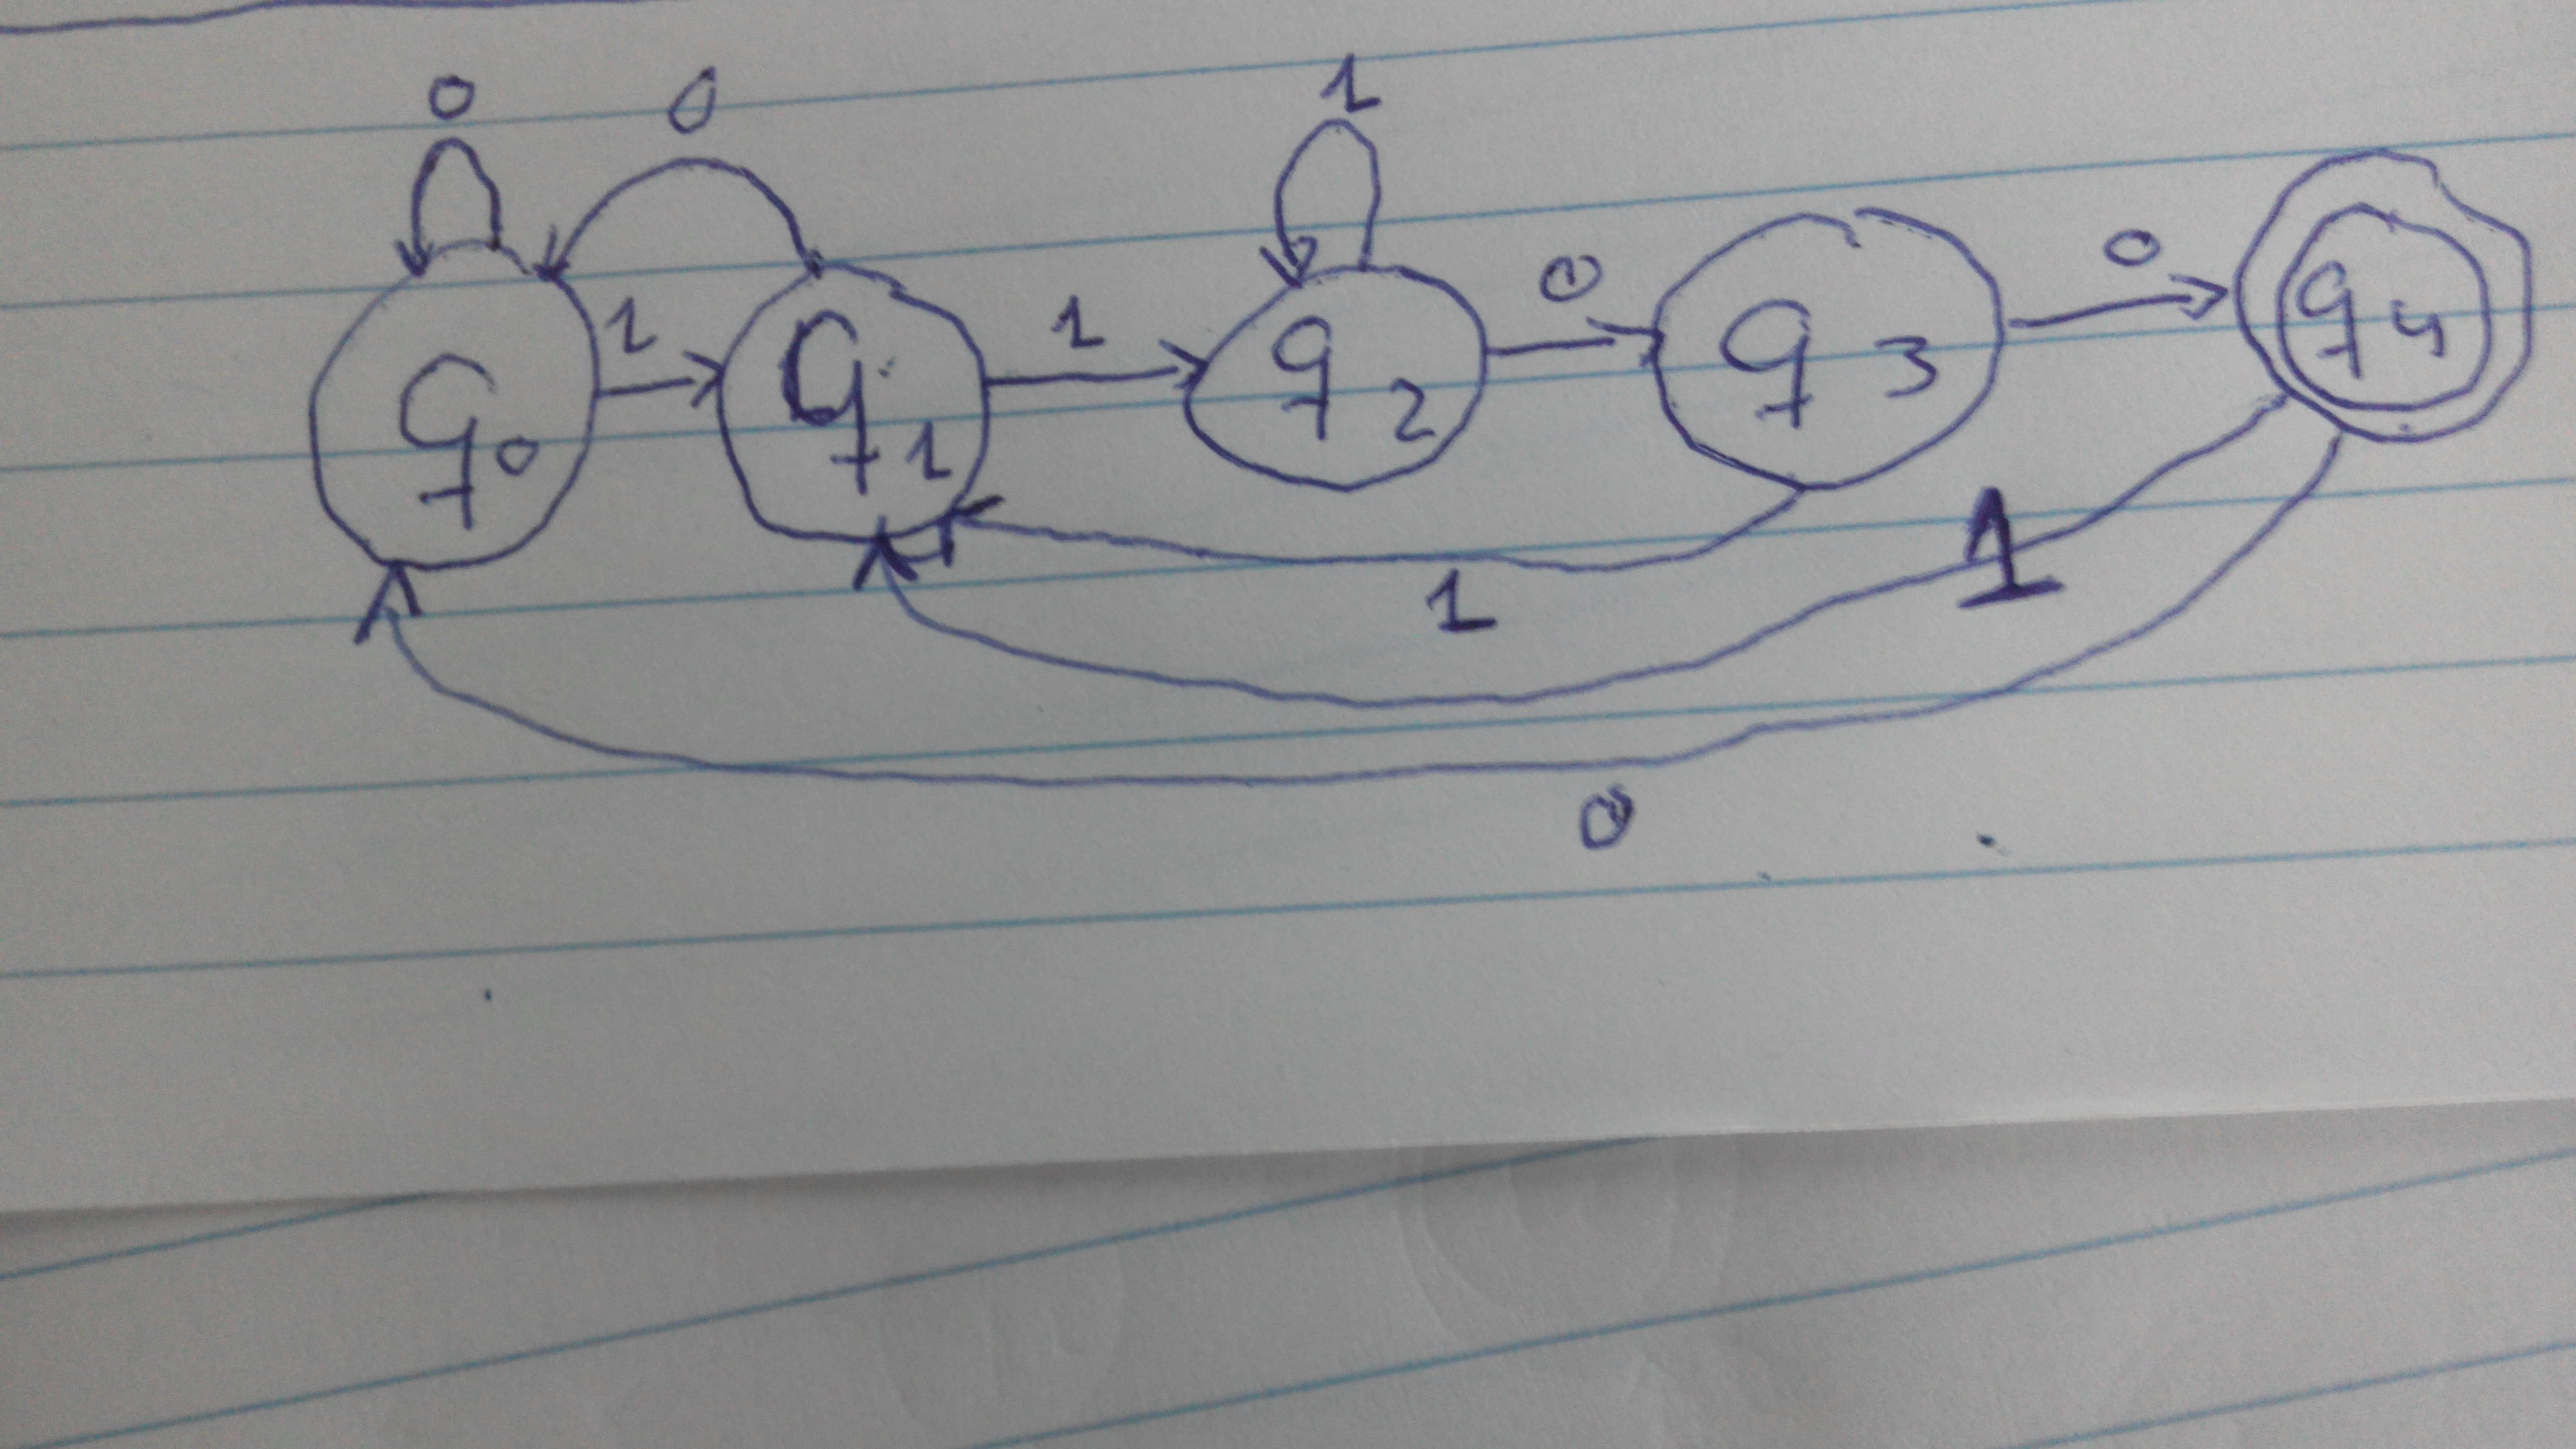
\includegraphics[width=7cm, height=5cm]{2}
        \end{figure}
  \item [3]·
        \begin{figure}[H]
          \centering
          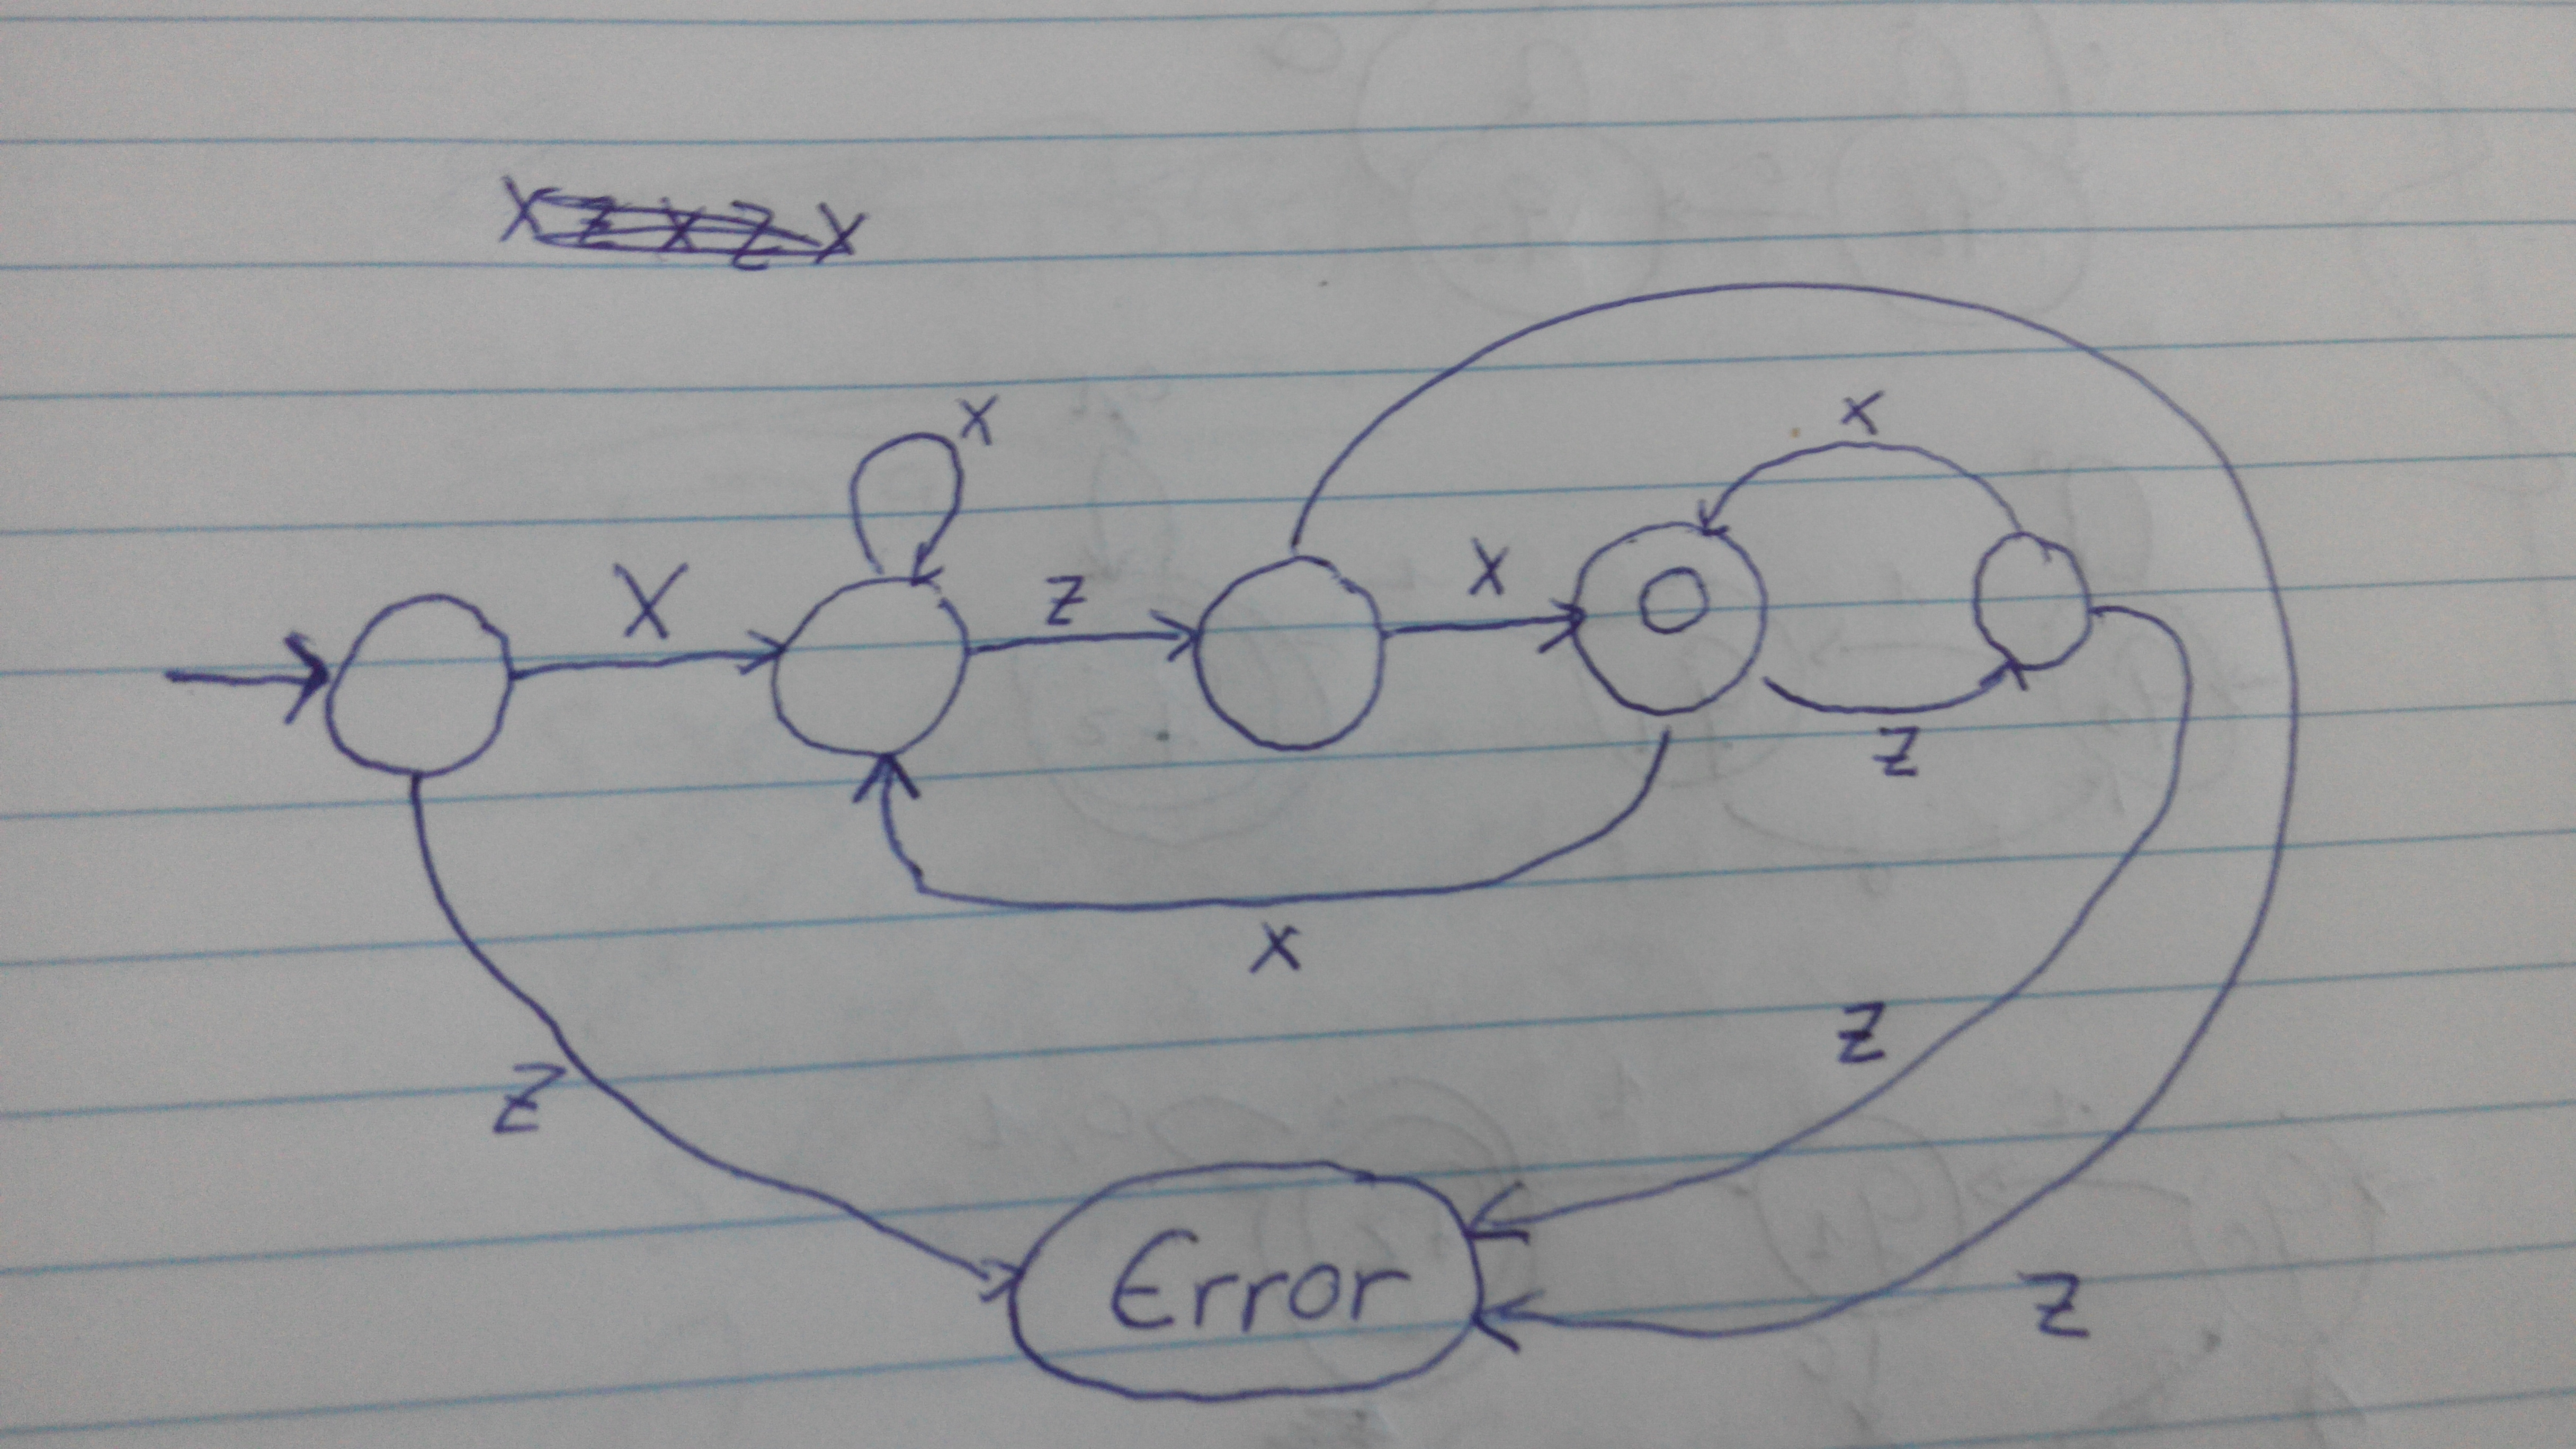
\includegraphics[width=7cm, height=5cm]{3}
        \end{figure}
\end{enumerate}


\end{document}
